\begin{example} \label{eg:5.6.1} % EXAMPLE
Approximate $\ds \int_0^1e^{-x^2}\ dx$ using the Left and Right Hand Rules with $5$ equally spaced subintervals.

\solution We begin by partitioning the interval $[0,1]$ into $5$ equally spaced intervals. We have $\dx = \frac{1-0}5 = 1/5=0.2$, so $$x_1 = 0,\ x_2 = 0.2,\ x_3 = 0.4,\ x_4 = 0.6,\ x_5 = 0.8,\ \text{and}\ x_6 = 1.$$

Using the Left Hand Rule, we have:

\begin{align*}
\sum_{i=1}^n f(x_i)\dx &= \big(f(x_1)+f(x_2) + f(x_3) + f(x_4) + f(x_5)\big)\dx \\
&= \big(f(0) + f(0.2) + f(0.4) + f(0.6) + f(0.8)\big)\dx \\
&\approx \big(1+0.961 + 0.852 + 0.698 + 0.527)(0.2)\\
&\approx 0.808.
\end{align*}

Using the Right Hand Rule, we have:

\begin{align*}
\sum_{i=1}^n f(x_{i+1})\dx &= \big(f(x_2) + f(x_3) + f(x_4) + f(x_5)+f(x_6)\big)\dx \\
&= \big(f(0.2) + f(0.4) + f(0.6) + f(0.8)+f(1)\big)\dx \\
&\approx \big(0.961 +0.852 + 0.698 + 0.527 + 0.368)(0.2)\\
&\approx 0.681.
\end{align*}

Figure~\ref{F:5-6-eg1} shows the rectangles used in each method to approximate the definite integral. These graphs show that in this particular case, the Left Hand Rule is an over approximation and the Right Hand Rule is an under approximation. To get a better approximation, we could use more rectangles. We could also average the Left and Right Hand Rule results together, giving $$ \frac{0.808 + 0.681}{2} = 0.7445.$$ The actual answer, accurate to $4$ places after the decimal, is $0.7468$, showing our average is a good approximation.
\end{example}

\begin{marginfigure}[-14cm] %MARGIN FIGURE
\subfloat[]{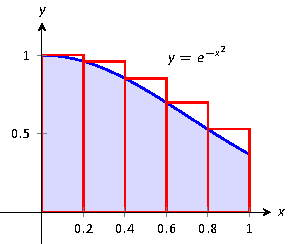
\includegraphics{figures/fignum1b}}

\subfloat[]{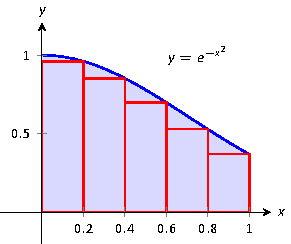
\includegraphics{figures/fignum1a}}
\caption{Approximating $\int_0^1e^{-x^2}\ dx$ in Example~\ref{eg:5.6.1}.}
\label{F:5-6-eg1}
\end{marginfigure}